% Chapter 3: RESULTS

\chapter{Results} % Main chapter title

\label{results} % For referencing the chapter elsewhere, use \ref{Chapter1} 

%%----------------------------------------------------------------------------------------
%
%% Define some commands to keep the formatting separated from the content 
%\newcommand{\keyword}[1]{\textbf{#1}}
%\newcommand{\tabhead}[1]{\textbf{#1}}
%\newcommand{\code}[1]{\texttt{#1}}
%\newcommand{\file}[1]{\texttt{\bfseries#1}}
%\newcommand{\option}[1]{\texttt{\itshape#1}}

%----------------------------------------------------------------------------------------

%PROVIDE A HIGH-LEVEL REVIEW, NOT LOTS OF NUMBERS

%REPRODUCABILITY OF WORK, i.e. make sure reader could redo it

%%----------------------------------------------------------------------------------------
%%----------------------------------------------------------------------------------------

Here, we will briefly explain the tool from a technical perspective, but more importantly  %and show how to use it in practice. %Additionally, we present an example of the tool in use.
we will present some highlights of the tool that sets it apart from other tools. In the appendix \ref{chp:manual} we guide the user through one example to illustrate how the tool is used in practice. This serves as a manual for users even though the steps are self-explanatory by just using the Graphical User Interface (GUI). 

Additionally, we will show some validation of the tool by comparing the angle computed by our tool to the one computed manually on 3 time-series image data sets of Arabidopsis roots.

The code is open-source and publicly available on \url{https://github.com/GiovanniSena/Auto-angle}; all previous versions including log files can be found on \url{https://github.com/burfel/root-tip-angle}.
%EMPHASISE THIS: MAKE RESEARCH TRANSPARENT


%COMMENTED OUT DUE TO WORD COUNT, goes into manual in appendix
%%----------------------------------------------------------------------------------------
%%----------------------------------------------------------------------------------------
%\section{Key features} %SHOW HOW ELEABORATE TOOL IS
%
%Figure [INSERT REFERENCE HERE: PIPELINE FROM GUI] explains the key components of this image-analysis software tool to address the problem of highly noisy electrotropism consumer camera images of Arabidopsis roots and a standardised way of computing the angle for the curved root tip. 
%
%This tool takes the form of a MATLAB program and subprograms with a graphical user interface on top of it.


%COMMENTED OUT DUE TO WORK OUT, shifted it down to "Components of GUI" section
%%----------------------------------------------------------------------------------------
%\subsection{Graphical User Interface}
%To make the program more user-friendly, we developed a graphical user interface (GUI). Pop-up windows, message boxes as well as error boxes, will guide the user through the process (see [INSERT REFERENCE HERE]); a separate manual is not necessary as the steps are very intuitive and straight-forward.
%There are various benefits of the GUI such as
%\begin{itemize}
%	\item Visualising the process including the pipeline and the angle that is computed
%	\item Easy user interaction with mouse clicking
%	\item Flexibility, e.g. the user can go back at each step without running the whole script from the beginning
%	\item Pop-up windows and mouseover functions on buttons that guide the user through the process and explain the steps
%	\item Error messages if user does not enter allowed values.
%\end{itemize}


%%----------------------------------------------------------------------------------------
%\subsection{Discerning root from background}
%
%Gamma correction (imadjust)
%[TO COMPLETE]


%COMMENTED OUT DUE TO WORD COUNT, goes into manual in appendix
%%----------------------------------------------------------------------------------------
%\subsection{Handling user's mistakes}
%
%When we take the user's input, e.g. choosing samples along the root, we correct for small mistakes by taking a neighbourhood (3\(\times\)3) average around the pixel. 
%%followed by adaptive thresholding.
%This means the user does not have to take special care when choosing the points as long as it is in the approximate region of the root.
%
%%----------------------------------------------------------------------------------------
%\subsection{User interaction and optional steps}
%The software tool was created in ways that it is easy to interact with for a future user. 
%We implemented several optional steps that only need to be performed if the user thinks they are necessary. This on the one hand saves time in the preprocessing but on the other hand also ensures that tricky roots can be tackled by various optional steps in order to extract a skeleton. 
%
%%----------------------------------------------------------------------------------------
%\subsection{Drawing the angle}
%The GUI lets the user visualise the angle that is computed. This not only helps to make the tool more visual and transparent, but can also assist in debugging. 


%----------------------------------------------------------------------------------------
%----------------------------------------------------------------------------------------
\section{Workflow of root skeletonisation}\label{sec:workflow}

For the skeletonisation part we chose a \textit{bottom-up} approach applying a sequence of filters to successively remove pixels considered unlikely to correspond to root material \cite{pound2013rootnav}. To achieve this we use common techniques like \textit{noise reduction}, \textit{thresholding}, i.e. selecting pixels above a given brightness or "threshold", and \textit{skeletonisation}, i.e. thinning selected groups of pixels down to lines of one pixel in diameter \cite{pound2013rootnav}. 

The pipeline that has been developed for the preprocessing step of extracting the skeleton of the root is displayed in figure \ref{fig:workflow} and can be viewed at the bottom of the GUI (explained in the next section), see chapter \ref{chp:manual}.
%In the appendix [INSERT REFERENCE HERE] we present the tool on one example image guides the reader through the pipeline and can serve as a manual for future users.

%[INSERT FIGURE OF DIFFERENT STEPS (SUBFIGURES) THAT ARE THEN REFERRED TO IN THE TEXT INDIVIDUALLY]

\begin{figure}[H]
	\centering
	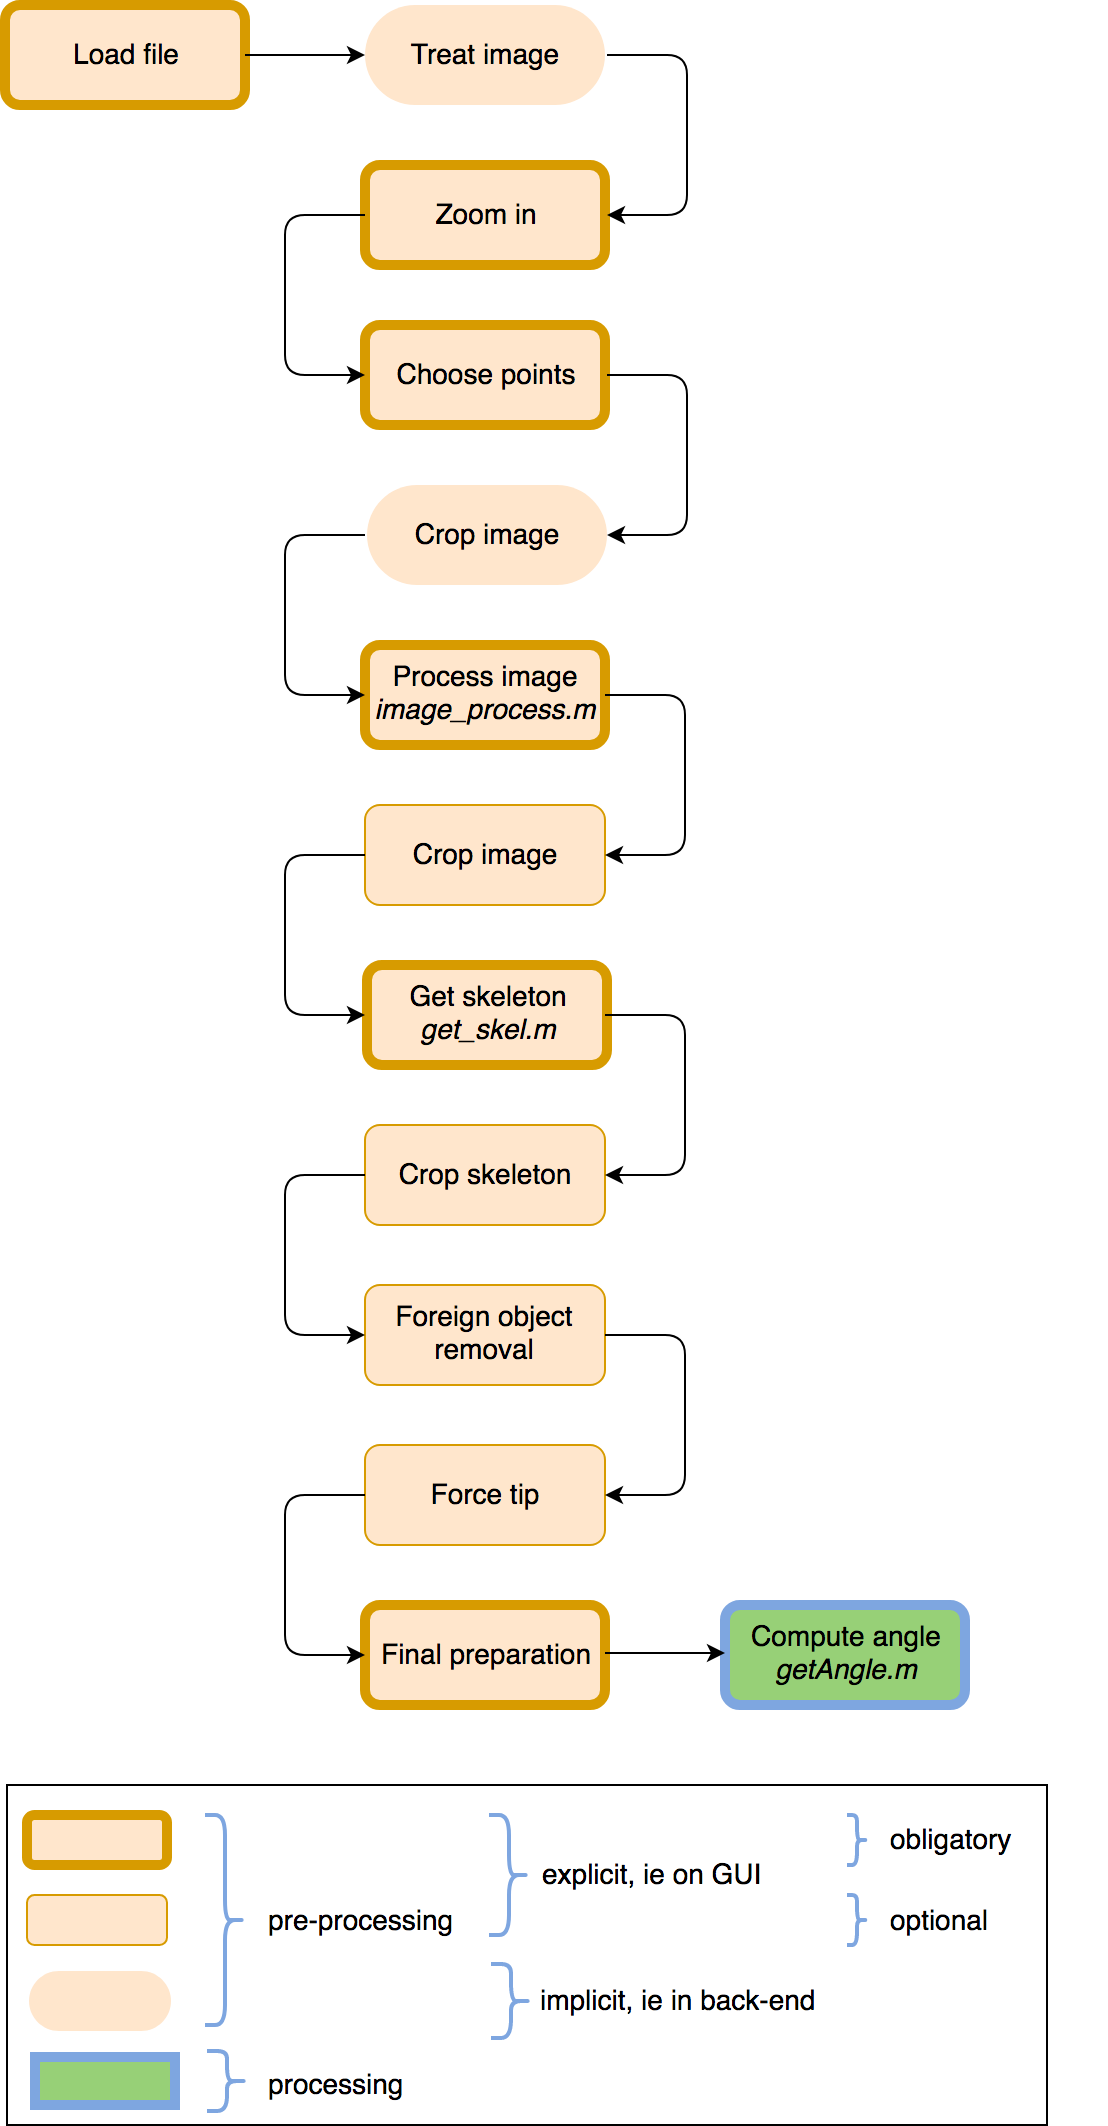
\includegraphics[width=0.78\textwidth]{../Figures/workflow_big.png}
	\caption{The workflow of \textit{RootSkel} and different components of the GUI: Pre-processing steps to extract the skeleton are highlighted in orange, the actual angle computation is shaded in blue. Steps that have a front-end, i.e. are visible on the GUI, are framed in red, only back-end components are without a frame. }
	\label{fig:workflow}
\end{figure}


%%%%%
%
%1) Treating the image 
%- multiplying to enhance contrast
%- gamma correction
%- adaptive thresholding
%- inverting image
%
%2) User draws a window around root of interest, samples 5-10 points of chosen root.
%Using the mean value and standard deviation of the pixel intensity of these points a thresholding range is found. Say [mu-3sigma,mu+3sigma]. 
%(Using the same threshold for all the images in the experiment was not successful as the noise patterns of the images vary too much.)
%
%
%3) Treating the cropped image using different filters
%
%Approach 1: Colour separation filtering 
%- based on RGB values of points
%- gray scales image
%
%Approach 2: Brightness filtering (intensity-based approach)
%- enhances brightness 
%- eliminates too bright spots
%
%4) SKELETONIZATION
%- unified approach (approach 1+2)
%
%5) Optional: additional cleaning
%- iteratively removing bigger and bigger connected objects (in steps of 30 pixels)



%%%%%%%%%%%%%%%%%%%%%%%%%%%%%%%%%%%%%%%%%%%%%%%%%%%%%%%%%%%%%%%%%%%%%%%%%%%%%%%
%%%%%%%-----WORK FROM HERE----%%%%%%%%%%%




%%%%%%%%%%%%%%%%%-----INCLUDE THIS------------
%%----------------------------------------------------------------------------------------
%\subsection{Loading a file}
%
%%----------------------------------------------------------------------------------------
%\subsection{Zooming in}
%
%and cropping
%
%
%%----------------------------------------------------------------------------------------
%\subsection{Choosing points}
%
%
%%----------------------------------------------------------------------------------------
%\subsection{Processing the image}
%
%Two approaches:
%1.
%Converted into gray channel images.
%2.
%
%
%%----------------------------------------------------------------------------------------
%\subsection{Optional image cropping}
%
%Additional cropping of the root ultimately solves the problem of getting rid of any artificial branches caused by noise close to the tip of the root.
%Also, the cropping does not have to be very accurate.
%
%
%%----------------------------------------------------------------------------------------
%\subsection{Extracting the skeleton}
%
%%----------------------------------------------------------------------------------------
%\subsection{Optional skeleton cropping}
%
%
%%----------------------------------------------------------------------------------------
%\subsection{Optional foreign object removal}
%
%Other than that, the user can perform iterative cleaning that gradually gets rid of those artificial branches (most of the times) as well; one has to be careful not to "loose" the root completely, but the user can undo the last cleaning step. 
%
%%----------------------------------------------------------------------------------------
%\subsection{Optional tip forcing}
%
%
%%----------------------------------------------------------------------------------------
%\subsection{Final preparation}
%
%
%%----------------------------------------------------------------------------------------
%\subsection{Angle computation}
%%%%%%%%%%%%%%%%%%%%%%%------INCLUDE THIS


%0) Convert the image from rgb to gray scale (matlab: rgb2gray) (3-tensor to matrix)
%
%intensify the matrix \arrowvert distinguish roots for user
%highlight window \arrowvert help user where approximately roots are

%
%1. The user will select a region of interest on the image so only roots appear. This window can be used over the whole experiment (as camera doesn’t move) ///TODO: or better to define window for each root?
%
%2. The user then clicks on some points over the roots (I'd say at least 7, preferably 10). Using the mean value and standard deviation of the pixel intensity of these points a thresholding range is found. Say [mu-2sigma,mu+2sigma]. 
%Initially trying to use the same threshold for all the images in the experiment, maybe this will do the job already…
%
%3. After segmenting the images, the binary images need to postprocessed so we get rid of the bright spots and noise, e.g. by removing any object that has fewer than 1000 pixels (matlab: bwareaopen enough?). Then any holes that might appear in the roots need to be filled (matlab: imfill)

%
%4. Hopefully obtaining the skeleton version of the binary image (matlab: bwmorph).
%
%5. Label each individual object in the image so they can later be processed independently (matlab: bwconncomp).

%6. For each root we then get the list of point belonging to the tip (upper x- and y-values) and we compute the curvature (e.g. on a 3-point polygonal chain)


%----------------------------------------------------------------------------------------
%----------------------------------------------------------------------------------------

%----------------------------------------------------------------------------------------
\section{Graphical User Interface}
To make the program more user-friendly, we developed a graphical user interface (GUI). Pop-up windows, message boxes as well as error boxes, will guide the user through the process (see chapter \ref{chp:manual}); a separate manual is not necessary as the steps are very intuitive and straight-forward.
There are various benefits of the GUI such as
\begin{itemize}
	\item Visualising the process including the pipeline and the angle that is computed
	\item Easy user interaction with mouse clicking
	\item Flexibility, e.g. the user can go back at each step without running the whole script from the beginning
	\item Pop-up windows and mouseover functions on buttons that guide the user through the process and explain the steps
	\item Error messages if user does not enter allowed values.
\end{itemize}


With the development of the GUI, we split our source code of the tool based on functionality, i.e. we create separate functions or modules that we then connect to several objects in the GUI. This process, also known as \textit{modularity} in software engineering, has various benefits for developing and maintaining the application: The code is less cluttered but more structured and readable and just by reading the main functions which calls all other subfunctions you get a general overview and understanding of what the code does. Also, it reduces redundancy in the main code if the code gets split up into smaller subfunctions and helps debugging. A clear naming convention also adds to a better understanding of the code.

%MODULARITY — main code is not as cluttered, things that are called again and again, migrate it. several functions use same code. 
%REDUCE REDUNDANCY
%MORE READIBLE, CLEARER, MORE STRUCTURED, DON’T GET LOST IF YOU ONLY READ MAIN CODE, GENERAL THIGNS THAT HAPPEN.
%SPEAKING VARIABLES. 


%Beyond that, provided the interface, i.e. input and output of each modules, is well defined modularity allows a team of developers to work on the functionality of one single module without involving other modules. They are not distracted by functionalities that are not relevant, known as information hiding in software engineering. Also, it helps to keep the code short and simple and focused one core functionality. It is also useful to identify bugs early on in the development process.

Here, it allowed us to not only handle front-end and back-end but also the different steps in the pipeline separately: 

Every function representing one specific step in the pipeline or objects accessed by various functions is encoded in the back-end which is not visible and relevant for the future user. These modules are connected via callbacks to different objects in the GUI which represent the front-end, see figure \ref{fig:fronendBackend}.


\begin{figure}[H]
	\centering
	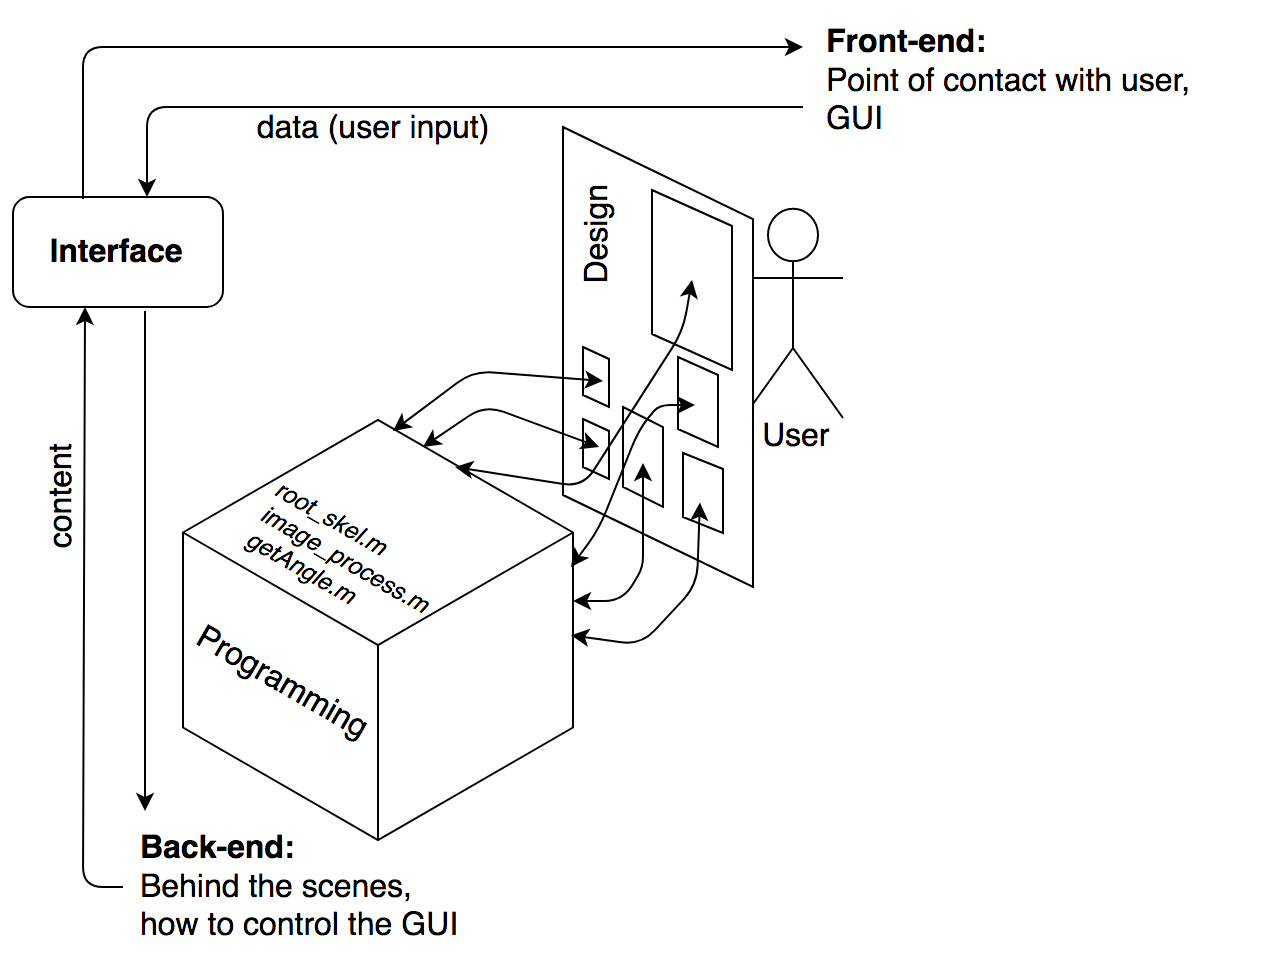
\includegraphics[width=1.\textwidth]{../Figures/frontBack.png}
	\caption{A scematic figure visualising how back-end and front-end communicate via a well-defined user interface: The back-end containing all the programs acts behind the scenes and controls the GUI; it sends content to the interface that get than transferred to the front-end. The front-end being the point of contact with the user contains the GUI and the design sends the user input data via the interface to the back-end.}
	\label{fig:fronendBackend}
\end{figure}


%Back-end as well as front-end needs maintaining. 
%The line between the two of them is often blurry.
%
%Front-end: involved with what the user sees, including design. 


Table \ref{table:modules} gives an overview of the different components and modules our software tool \textit{RootSkel} consists of. It has been developed over a cycle of various iterations, together with an exemplary future user. 
%The current version of the package can be downloaded from [INSERT REFERENCE HERE]. %https://github.com/burfel/root-tip-angle/tree/master/src/Root_image_GUI_v1_5 and will be maintained on [INSERT GIOVANNIS GITHUB HERE].



%image_process.m
%* extracts the cropped image 
%* extracts the colours from the sample pixels, averages it with a certain neighbourhood
%* takes a brightness range, an average of the three filters used 
%* approach 1: using input from the user to estimate the range of the root colours
%* initial colour filtering based on the RGB values of the selected points
%* subsequent gray filtering
%* RGB level difference based filtering
%* …….
%* approach 2: using brightness filter (intensity based)
%* Idea: We carefully enhance the brightness and then get rid of too bright spots.
%* gray scaling
%* creating a filtering mask according to the brightness rank



%MAYBE USE STH FROM HERE BUT COMMENTED OUT FOR NOW, AS WIDELY REPETITION:
%Even though most of image processing work is empirical, i.e. based on trial and error and educated guesses on the given data set, we try to explain why certain features were necessary to implement. %this explanations are marked in italics.
%The pipeline can be seen in the at the bottom of the GUI in figure [INSERT REFERENCE HERE].
%
%[INCLUDE IN GRAPHIC IF EXCEED WORD COUNT]
%
%%1. Open file
%%2. Zoom in
%%3. Choose Points
%%4. Process image
%%5. Crop image (optional): 
%%6. Get skeleton
%%7. Crop skeleton (optional): It allows the user to crop a region around the skeleton by hand to definitely remove things outside the region of interest. The user can redo the cropping in case she is not satisfied. 
%%8. Foreign object removal (optional): It allows the user to remove objects, i.e. if the skeleton contains undesired branches. The user can undo the last cleaning step in case the root gets removed in the last step, to not start the entire process again. 
%%9. Force tip (optional)
%%10. Final preparation
%%
%%The bar on the left shows various other buttons that allow the user to perform other functions:
%%* In the upper part: 
%%* Save variables
%%* Save figures: select the cropped image or the skeleton; both are greyed out as longs as objects have not been created
%%* Load variables
%%* Load figure: choose one of the radio buttons either on the left or on the right
%%* In the middle part: 
%%* Show skeleton; greyed out as long as the skeleton has not been created
%%* Clear figure: choose one of the radio buttons either on the left or on the right
%%* The bottom part to compute and display the angle:
%%* Using user’s point
%%* Using curvature
%
%The GUI includes helpful text along the pipeline as well as pop up windows including instructions or warnings in case the user does not follow them. 
%
%In the appendix [INSERT REFERENCE HERE] we guide the user through the different steps of the pipeline and present one example each; this can serve as a manual for users even though the steps are rather self-explanatory by just using the GUI. Also, having a GUI rather than a script with pop-up-windows not only makes the tool more visually attractive but it one can also repeat a step without restarting the whole process or script again. This all adds to the user-friendliness.

%----------------------------------------------------------------------------------------
%----------------------------------------------------------------------------------------
\section{Validation: Comparing the automated calculated angles with the manually calculated angles}

As a preview of validation we performed our software tool on 3 randomly chosen roots from 3 different experiments over a time of 330 minutes (or 100 minutes respectively). We compared both the automatically computed angles with the previously computed manual angle. As a second validation layer we also compared the latter to the computed angles with the turning point as user input.

Figure \ref{fig:resultPlots} shows the comparison of the angle of interest \( \Theta \), both of the manual as well as the automatically computed angle at about 11 times steps over a period of 330 minutes.

%\begin{figure}[H]
%\centering
%\includegraphics[width=0.6\textwidth]{Figures/2018-04-24.png}
%\caption{}
%\label{fig:2018-04-24}
%\end{figure}

%\begin{figure}
%	\begin{subfigure}
%		\includegraphics[]{../Figures/2018-04-24.png}
%	\end{subfigure}
%	\begin{subfigure}
%		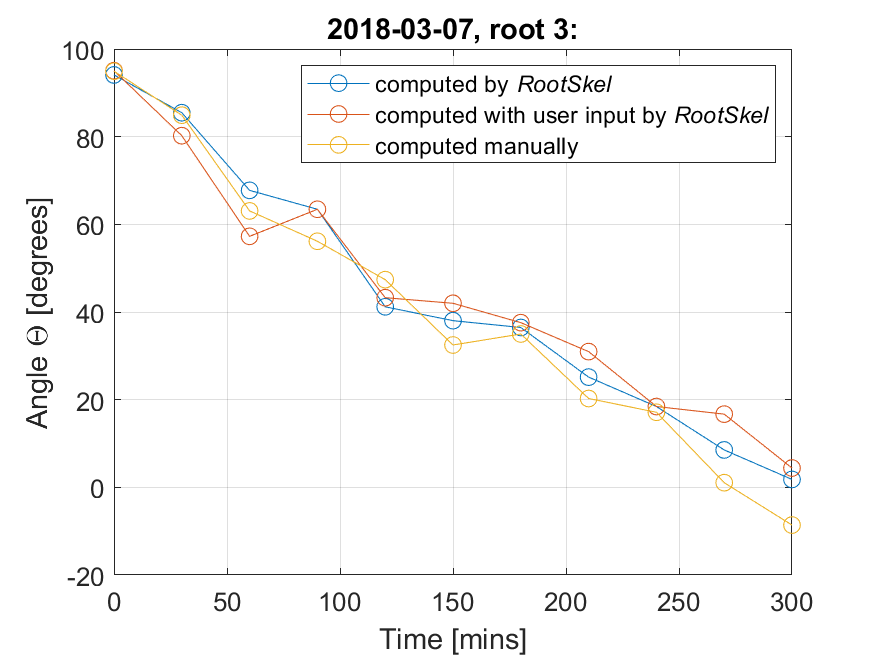
\includegraphics[]{../Figures/2018-03-07.png}
%	\end{subfigure}
%	\begin{subfigure}
%		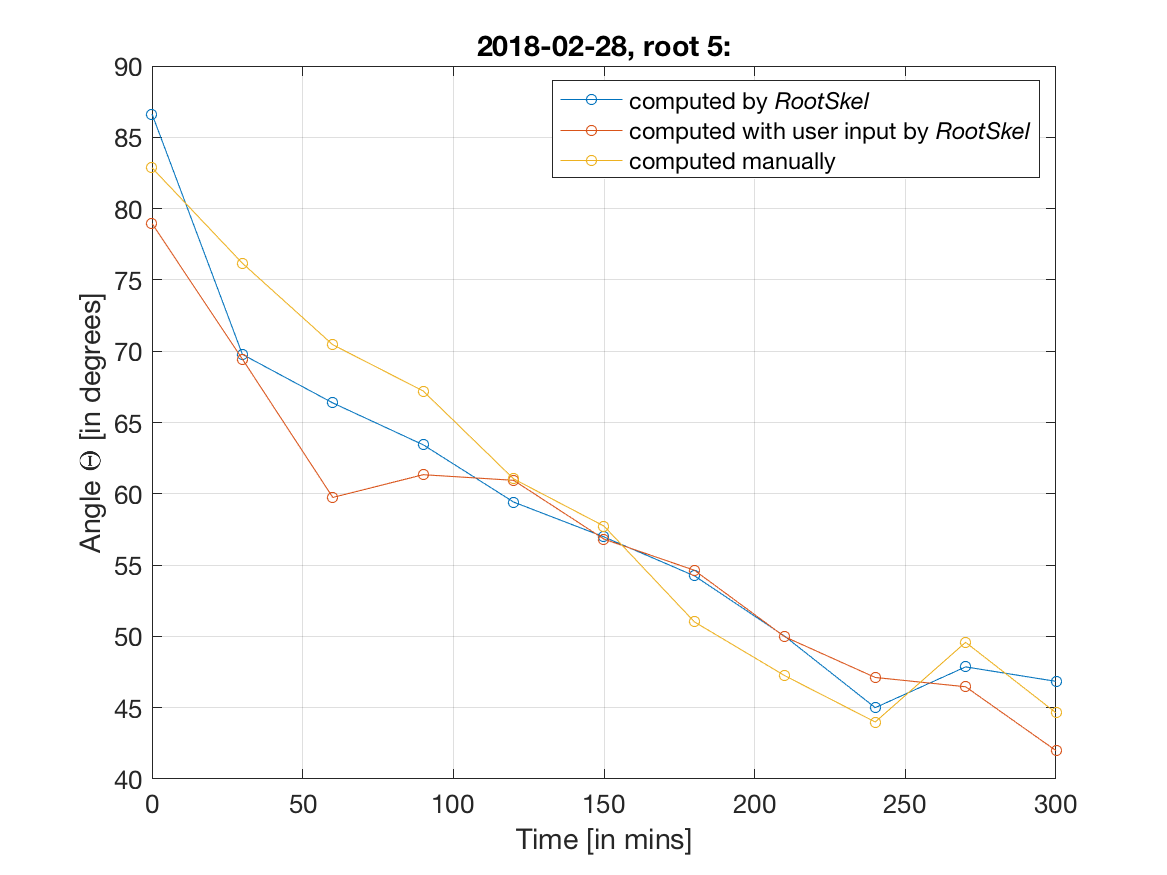
\includegraphics[width=\textwidth]{../Figures/2018-02-28.png}
%	\end{subfigure}
%\end{figure}

%\newpage

\begin{figure}[H]

\centering

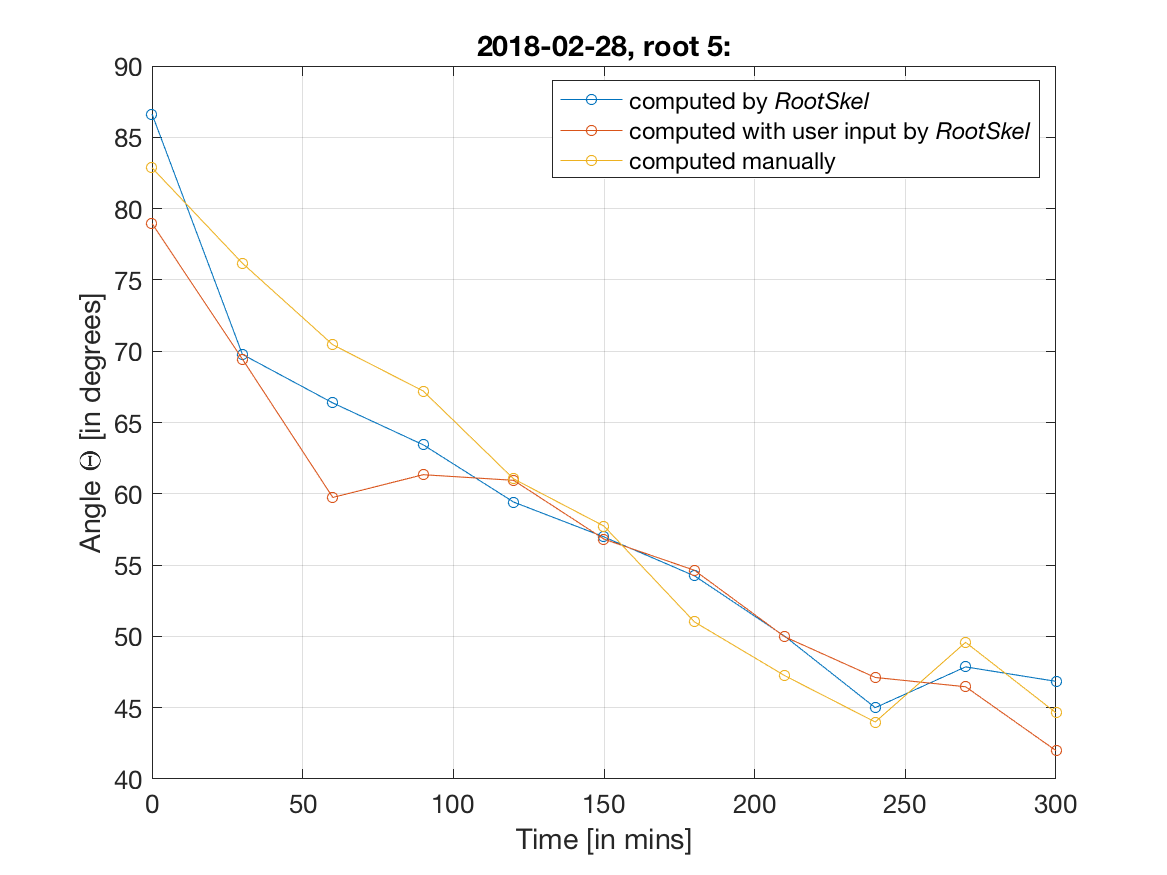
\includegraphics[width=.65\textwidth]{../Figures/2018-02-28.png}
%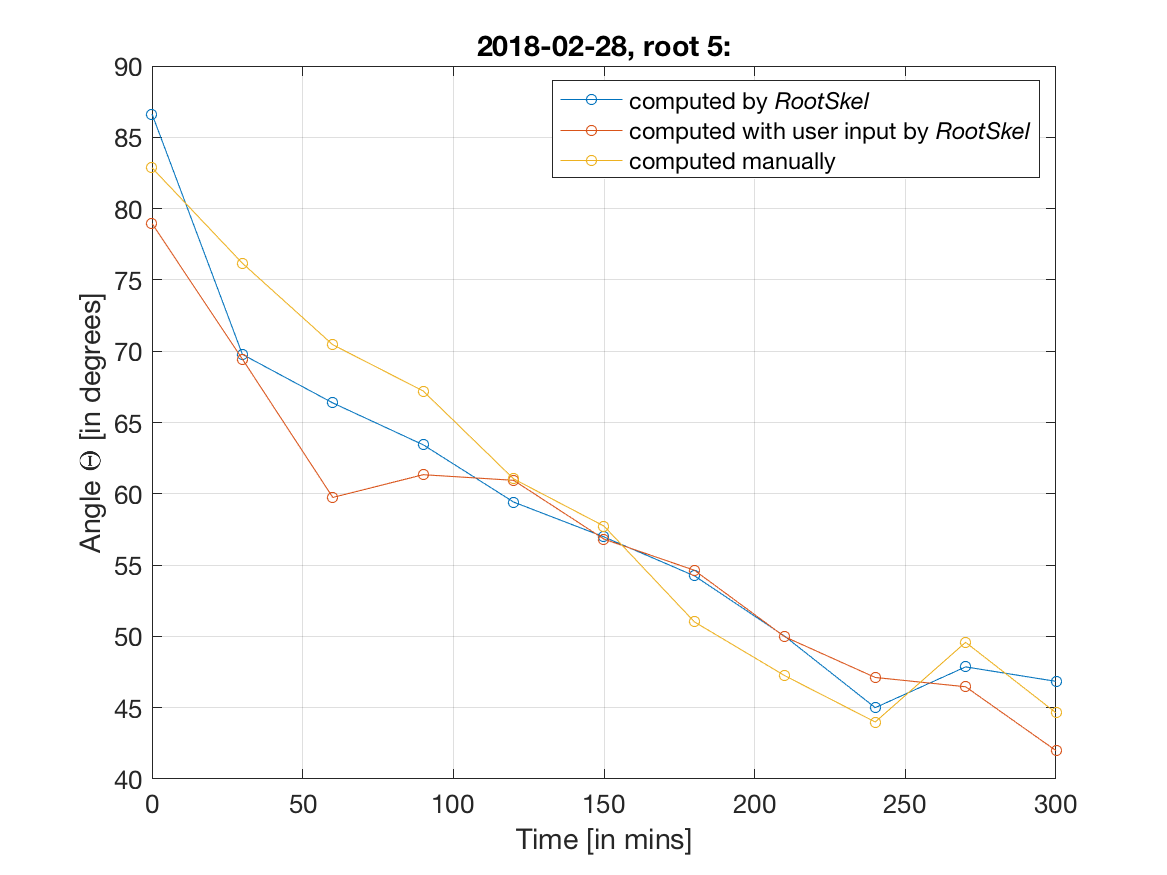
\includegraphics[width=150mm,scale=15]{../Figures/2018-02-28.png}

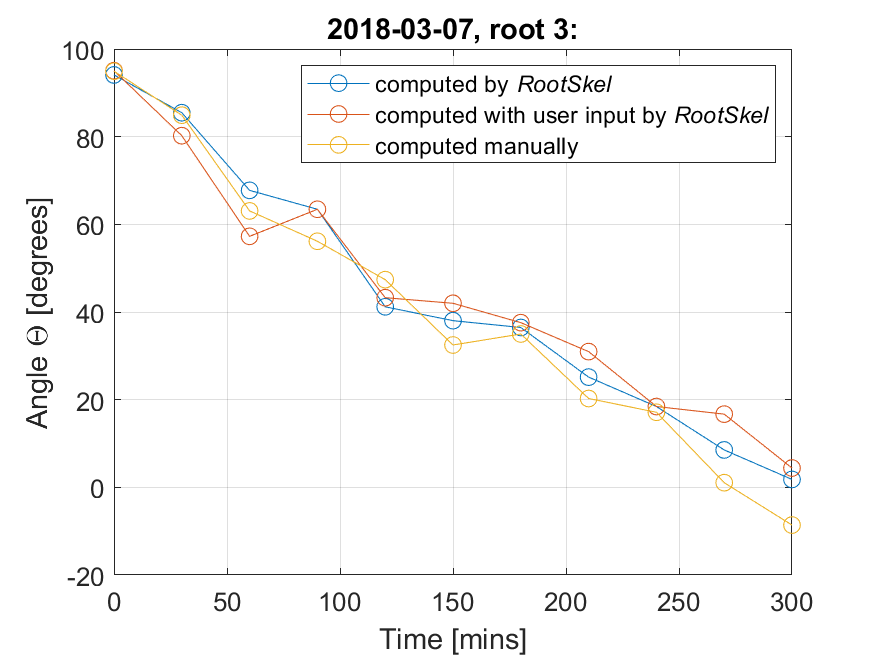
\includegraphics[width=.65\textwidth]{../Figures/2018-03-07.png}

\includegraphics[width=.65\textwidth]{../Figures/2018-04-24.png}

	\caption{Comparing the manually computed angle and the angle(s) computed by \textit{RootSkel}; in blue: computed by \textit{RootSkel}, in red: computed by \textit{RootSkel} with the turning point as user input, in yellow: manually computed angle. Each plot is labelled by the data set it was taken from (named after date) and the root number (starting from the left hand side in an image). Computations of all three approaches exhibit similar patterns; the angle \( \Theta \) continuously decreases. %Differences between the three approaches are in the magnitude of 5 degrees, single points vary up to 12 degrees, see also figure [INSERT REFERENCE HERE].
		}
\label{fig:resultPlots}
\end{figure}


Differences between the three approaches are in the magnitude of 5 degrees, single points vary up to 12 degrees, see also table \ref{table:resultTable}.
Table \ref{table:resultTable} compares the automatically computed angle by \textit{RootSkel} with the manually computed angles of the 3 roots. We compute the absolute difference in the angles and introduce an \textit{improvement score} defined as 
\[
 \text{score}_{\textbf{imp}} := | \frac{ \alpha_{\text{RootSkel}} - \alpha_{\text{manual}} }{\alpha_{\text{manual}}} |
\]
where $\alpha_{\text{RootSkel}}$ denotes the angle computed by \textit{RootSkel} and $\alpha_{\text{manual}}$ denotes the manually computed angle; this way we compare to the manually computed angles. How much our method is really an improvement (in accuracy) to the manual method, i.e. how much closer it is to the theoretical true value, cannot be computed as any measurement will be subject to errors (see also section \ref{sec:validation}). The improvement score on our 3 example data sets average between 5\% and 23\% with an ensemble average of 12.4\%, which can be concluded from table \ref{table:resultTable}.

When studying our data sets (manually computed and automatically computed angles), we could observe that as the angle approaches zero, the values get more volatile, i.e. the variance increases; this matches up with our observations presented in figure \ref{fig:resultPlots}. However, it should be noted that our improvement score is based on relative values and, therefore, can easily increase for small values. %(of manually computed angles and increasing or constant difference/ variance to the automatically computed angle).


\begin{table}[H]
	\centering
	%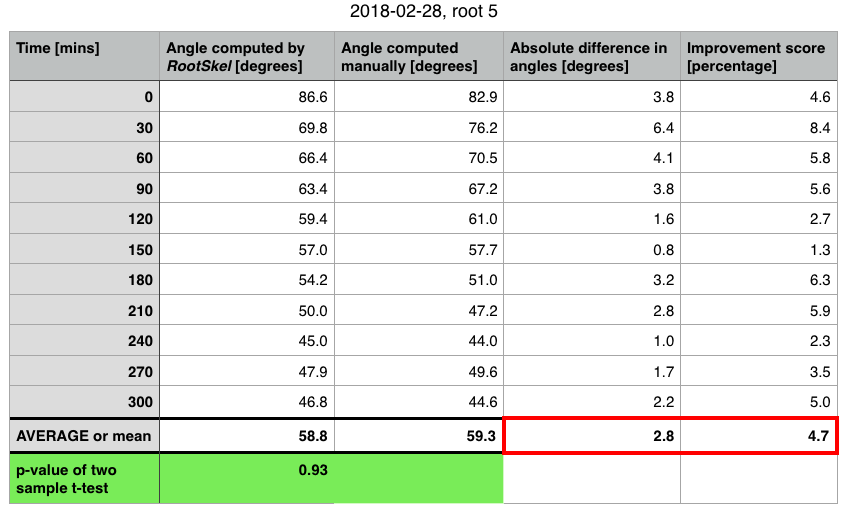
\includegraphics[width=.7\textwidth]{../Figures/2018-02-28-stats-new.png}
	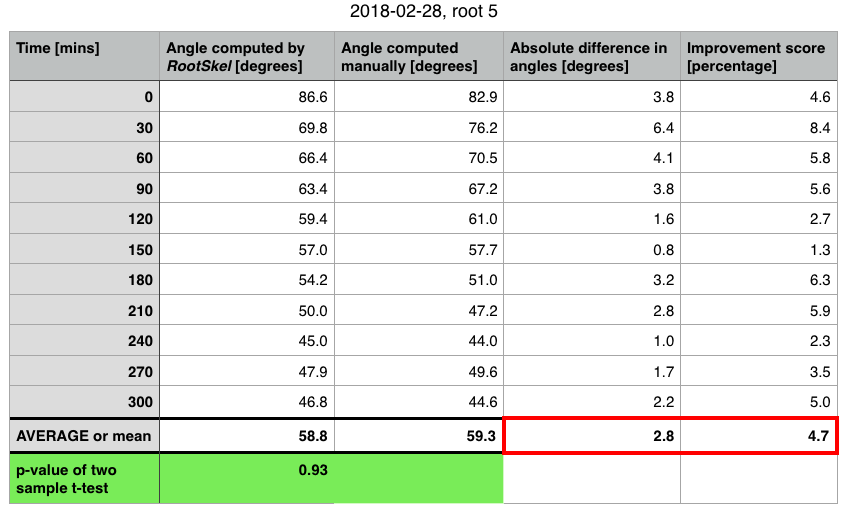
\includegraphics[width=\textwidth]{../Figures/2018-02-28-stats-new.png}
	%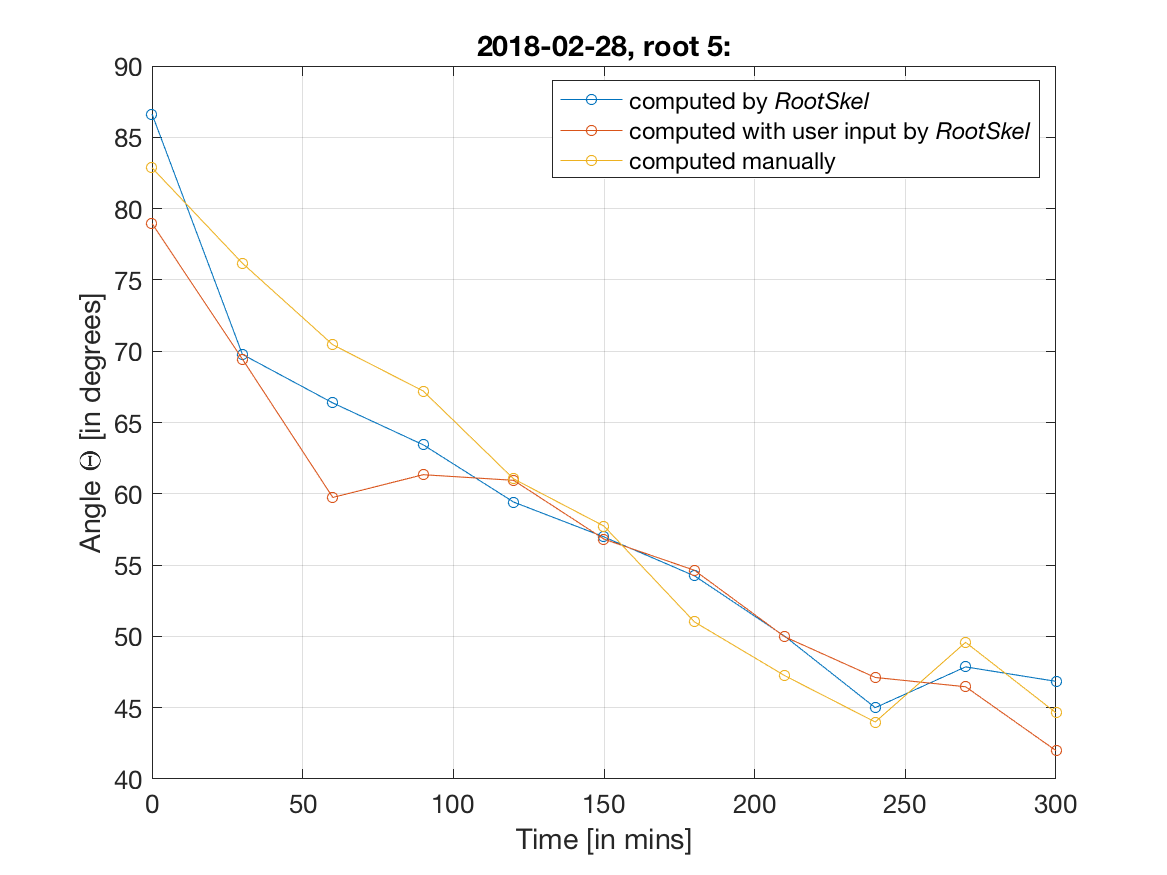
\includegraphics[width=150mm,scale=15]{../Figures/2018-02-28.png}
	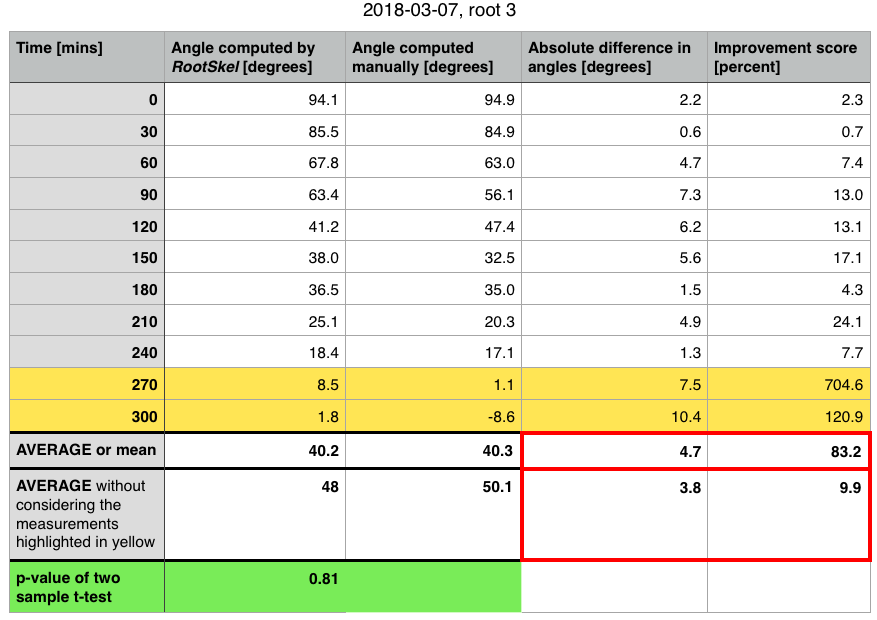
\includegraphics[width=\textwidth]{../Figures/2018-03-07-stats-new.png}
	\caption{Comparing the automatically computed angle by \textit{RootSkel} with the manually computed angles on the 3 roots. Average values of the difference in the angles and the improvement score are highlighted by a red margin; values that highly skew the results and are advised to be left out when doing the average calculations are highlighted in yellow.
	The p-values of a two sample t-test are highlighted in green.\\ 
	It should be noted that we made an educated estimation of the measurement error, i.e. the total error, to be about about 5\% of our computed \textit{RootSkel} value. We round this error to two significant digits according to convention and computed the absolute difference in the angles and the improvement score with this precision; we only round once we present the values to avoid rounding errors. }
	\label{table:resultTable}
\end{table}
\begin{table}[H]
%	\newpage
	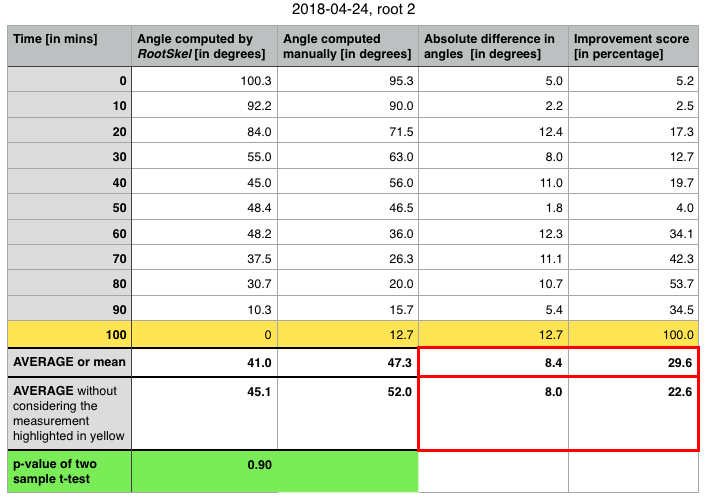
\includegraphics[width=\textwidth]{../Figures/2018-04-24-stats-new.png}
	\caption{See table \ref*{table:resultTable}.}
	\label{table:resultTable2}
\end{table}


As a validation that the computed values of \textit{RootSkel} are similar enough to the manually computed values, we perform a t-test between the two sets of angles.
In all three cases we fail to reject the null hypothesis (at a 95\% confidence interval), implying that the difference between each of the two samples is not statistically significant. The p-values of the two sample t-tests can be found in tables \ref{table:resultTable} and \ref{table:resultTable2}.

%we fail to reject the null hypothesis. So we are not "rejecting the null", implying that we don't have enough evidence to assume that the difference in means is different from zero.

%We assume there is no difference, and since the t-score with p-value is larger than 0.05 we cannot reject this hypothesis, i.e. the difference between the two samples is not statistically significant; this does not mean there is no difference that can be relevant in statistics.


%We show that there is no significant difference between the two sets of values. 

%Kolmogorov Smirnov test is independent of distribution and would be suitable for your data.

%FOR VIVA: Alternatively, we could ask how similar the two data sets are and perform a \( \Chi^{2} \) test; 
% tests for strenght of association between the two variables.
%If it was due to chance we would see it in 23\%.


%The variance of the angle pairs is shown in figure [INSERT HERE]. Performing a t-test we can conclude that the improvement of the angle computation accuracy is significant. Approximately [INSERT HERE] \% due to human error can be eliminated.
%%Looking at the variance of the angle pairs and performing a t-Test, we can conclude that by our tool we can minimise the human error by [INSERT HERE]\%. 
%
%Once more angles have been compared, more confident statistics can be obtained. 
%
%[INSERT FIGURE HERE]



